\chapter{Numerical results}\label{chapter:numerical-results}
In this chapter we present a numerical example to showcase the ideas introduced earlier.
As the reference domain, we consider the three-dimensional unit cube $D_{\text{ref}} = (0,1)^3$.
The eigenvalues of \eqref{eq:og-prob} on the reference domain are given by 
\[
    \lambda_k = \pi^2(k_1^2+k_2^2+k_3^2)
\]
with associated eigenfunctions
\[
    u_k(x) = \sin(\pi k_1 x_1)\sin(\pi k_2 x_2)\sin(\pi k_3 x_3)
\]
for all $k = (k_1,k_2,k_3)\in \bN^3$.

For modeling the domain and computing the solution of (\ref{eq:og-prob}), we employ the \texttt{C++} library \texttt{bembel} \cite{Bembel2020}.
We want to find mean values for the eigenvalues $\lambda_k$ where $\kappa_k = \sqrt{\lambda_{k}}$ is located inside of the ellipse with center $\mu = \frac{(\sqrt{3}+\sqrt{6})\pi}{2}$, width $2a = 4$ and height $2b = 0.4$.
The ellipse can be parametrized by $\varphi(t) = \mu + \frac{a+b}{2}e^{it} + \frac{a-b}{2}e^{-it}$ for $t\in [0,2\pi]$.
In the reference case, the contour contains $\kappa_{(1,1,1)} = \sqrt{3}\pi, \kappa_{(1,1,2)} = \kappa_{(1,2,1)} = \kappa_{(2,1,1)} = \sqrt{6}\pi$.
In order to ensure that the eigenvalues stay separated by our contour over the entire parameter space, we scale it by $\alpha = \frac{1}{3}$, i.e. we only take random parameters $\boldsymbol{y} \in [-\frac{1}{3},\frac{1}{3}]^\bN$ instead of  $\boldsymbol{y} \in [-1,1]^\bN$. In practice, we approximate this by $\boldsymbol{y} \in [-\frac{1}{3},\frac{1}{3}]^N$ with $N$ large enough.
\begin{figure}
    \centering
    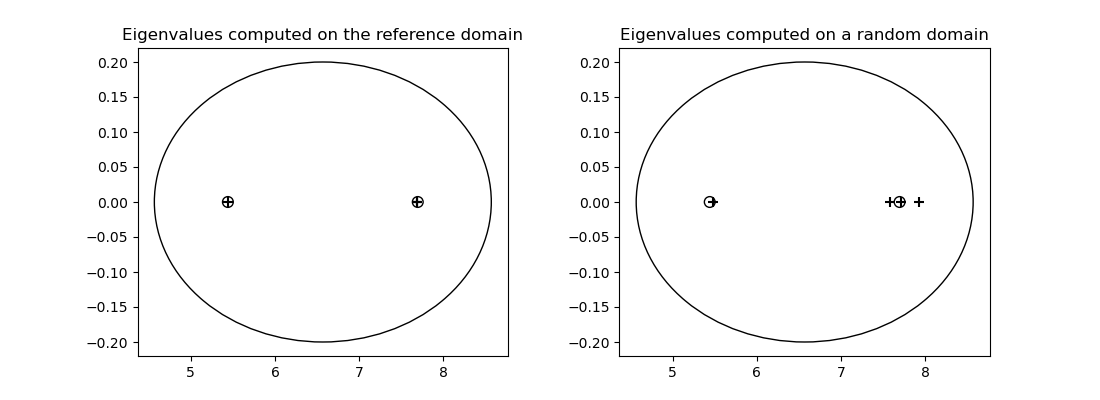
\includegraphics[width=\textwidth]{chapter_numerical_results/both_new_ratio_new_size.png}
    \caption{Two realizations of the contour integral method for a Galerkin approximation (polynomial degree zero and refinement level three) of the single layer boundary integral operator. The open circles indicate the exact eigenvalues on the reference domain, the crosses the approximations computed by the contour integral method.}
    \label{fig:cim}
\end{figure}
\Cref{fig:cim} contains two results of the contour integral method, one on the reference domain and one on a random perturbation of the domain. They show that indeed a bifurcation occurs, as on the reference domain we have an eigenvalue with multiplicity three, while for the random domain we find four different simple eigenvalues.

As we are integrating over a high-dimensional parameter space, we use a multilevel quasi-Monte Carlo quadrature (QMC) with the Kronecker sequence \cite{Dick_Kuo_Sloan_2013}.
Due to the asymptotic convergence rate of $h^{2p+3}$ of the boundary element method for the approximation of the eigenvalues, the number of samples for the quadrature has to be adapted for each level according to $\sim h^{-2p-3}$.
This yields the number of quadrature points as shown in \Cref{tab:number-of-samples}.

\begin{table}[htb]
    \centering
\begin{tabular}{c c c c c}
    \hline
     & $\ell=2$ & $\ell=3$ & $\ell=4$ & $\ell = 5$ \\\hline
    $p = 0$ & 5\,120 & 640 & 80 & 10 \\\hline
    $p = 1$ & 10\,240 & 320 & 10 &  \\\hline
    \end{tabular}
    \medskip
    \caption{Number of samples on the different levels for QMC.}
    \label{tab:number-of-samples}
\end{table}

In order to measure the approximation errors, we compute a reference solution on the finest level for each polynomial degree using a quasi-Monte Carlo method with the Halton sequence \cite{Dick_Kuo_Sloan_2013}.
The error is given in terms of the $\ell^{\infty}$-norm calculated with respect to the eigenvalues, that is, we take the error to be $\max_{i=1,\ldots,k} \abs{\lambda_i^{L} - \lambda_i^{\text{ref}}}$, where $\lambda_1^{L},\ldots,\lambda_k^{L}$ are the eigenvalues of the approximation $\mathcal{Q}_L^{\text{ML}} [B]$ and $\lambda_1^{\text{ref}},\ldots,\lambda_k^{\text{ref}}$ are the eigenvalues of our reference solution for $\bE[B]$.

\begin{figure}
    \centering
    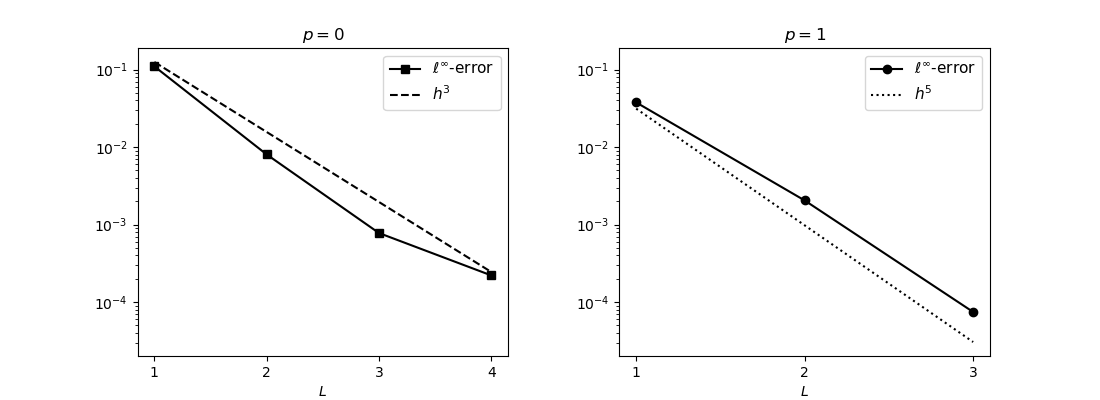
\includegraphics[width=\textwidth]{chapter_numerical_results/plots_new_ratio.png}
    \caption{Convergence of multilevel QMC for the expectation of the eigenvalues. \textit{Left}: Using a BEM with piecewise constant functions. \textit{Right}: Using a BEM with piecewise linear functions.}
    \label{fig:plots}
\end{figure}
\Cref{fig:plots} illustrates the results obtained, where the dashed lines indicate the expected convergence rate of the boundary element method.
We see that the results seem to confirm the theoretical error estimates.
The bend in the error plot where we used piecewise constant approximation spaces could be ascribed to lacking accuracy of our reference solution.
Alas, due to the large number of samples and the high computational cost of evaluating the single layer boundary integral operator, more approximations as well as a better reference solution are out of reach with the available resources.